\documentclass[a4paper,12pt]{article}
\usepackage[margin=18mm]{geometry}
\usepackage{tikz}
\usepackage{amsmath}
\usepackage{xcolor}
\newcommand{\pFourCell}[2]{\makebox[#1em][c]{\ensuremath{#2}}}
\newcommand{\pFourCenterBox}[1]{\begingroup\setbox0=\hbox{$\displaystyle #1$}\dimen0=\ht0\advance\dimen0 by -\dp0\divide\dimen0 by 2\lower\dimen0\box0\endgroup}
\newdimen\pFourFractionRuleThickness
\pFourFractionRuleThickness=0.4pt
\newcommand{\pFourTopAlign}[3]{\raisebox{-#1}[0pt][\dimexpr #1 + #2\relax]{\ensuremath{\displaystyle #3}}}
\newcommand{\pFourBottomAlign}[3]{\raisebox{#2}[\dimexpr #1 + #2\relax][0pt]{\ensuremath{\displaystyle #3}}}
\newcommand{\pFourFractionInner}[2]{\hbox to #1{\hss$\displaystyle #2$\hss}}
\newcommand{\pFourFractionC}[4]{\begingroup\color{#1}\genfrac{}{}{\pFourFractionRuleThickness}{0}{\raisebox{0.14em}{\pFourFractionInner{#2}{{\color{black}#3}}}}{\raisebox{-0.18em}{\pFourFractionInner{#2}{{\color{black}#4}}}}\endgroup}
\newcommand{\pFourFraction}[3]{\genfrac{}{}{\pFourFractionRuleThickness}{0}{\raisebox{0.14em}{\pFourFractionInner{#1}{#2}}}{\raisebox{-0.18em}{\pFourFractionInner{#1}{#3}}}}
\newcommand{\pFourRootC}[2]{\begingroup\setbox0=\hbox{$\displaystyle #2$}\setbox2=\hbox{$\displaystyle \sqrt{\vphantom{\copy0}\hphantom{\copy0}}$}\dimen0=\wd2\advance\dimen0 by -\wd0\hbox{\rlap{\textcolor{#1}{\copy2}}\kern\dimen0\box0}\endgroup}
\newcommand{\pFourRoot}[1]{\pFourRootC{black}{#1}}
\newcommand{\pFourRootDegreeC}[3]{\begingroup\setbox0=\hbox{$\displaystyle #3$}\setbox2=\hbox{$\displaystyle \sqrt[#2]{\vphantom{\copy0}\hphantom{\copy0}}$}\dimen0=\wd2\advance\dimen0 by -\wd0\hbox{\rlap{\textcolor{#1}{\copy2}}\kern\dimen0\box0}\endgroup}
\newcommand{\pFourRootDegree}[2]{\pFourRootDegreeC{black}{#1}{#2}}
\pagestyle{empty}
\begin{document}

\section*{Spaltentreue LaTeX-Ausgabe}
\noindent Gleichung: \texttt{e}\texttt{\textasciicircum{}(2*}\texttt{x}\texttt{-1)=2/}\texttt{sqrt}\texttt{(2+}\texttt{a}\texttt{)  ->  2*}\texttt{x}\texttt{-1=}\texttt{ln}\texttt{(2/}\texttt{sqrt}\texttt{(2+}\texttt{a}\texttt{))} \hfill Zielvariable: \texttt{x} \hfill Profil: \texttt{standard}

\vspace{8mm}
\begin{center}
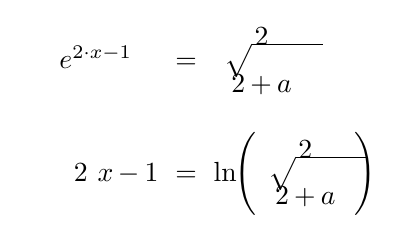
\begin{tikzpicture}[x=1em,y=-1em]
\node[anchor=base, inner sep=0pt] at (2.46,2.68) {$\pFourCell{4.92}{e^{{\scriptstyle 2\cdot{}x-1}}}$};
\node[anchor=base, inner sep=0pt] at (8.45,2.68) {$\pFourFraction{3.82em}{\makebox[3.82em][c]{\ensuremath{\pFourCell{0.88}{2}}}}{\makebox[3.82em][c]{\ensuremath{\pFourCell{0.88}{2}\pFourCell{0.78}{+}\pFourCell{0.9}{a}}}}$};
\node[anchor=base, inner sep=0pt] at (5.73,2.68) {$\pFourCell{1.62}{=}$};
\node[anchor=base, inner sep=0pt] at (8.89,2.68) {$\pFourCell{2.94}{\pFourRoot{\makebox[2.56em][l]{\rule[-0.28em]{0pt}{0.915em}}}}$};
\node[anchor=base, inner sep=0pt] at (10.03,6.76) {$\pFourFraction{3.82em}{\makebox[3.82em][c]{\ensuremath{\pFourCell{0.88}{2}}}}{\makebox[3.82em][c]{\ensuremath{\pFourCell{0.88}{2}\pFourCell{0.78}{+}\pFourCell{0.9}{a}}}}$};
\node[anchor=base, inner sep=0pt] at (1.92,6.76) {$\pFourCell{0.88}{2}$};
\node[anchor=base, inner sep=0pt] at (2.81,6.76) {$\pFourCell{0.9}{x}$};
\node[anchor=base, inner sep=0pt] at (3.65,6.76) {$\pFourCell{0.78}{-}$};
\node[anchor=base, inner sep=0pt] at (4.48,6.76) {$\pFourCell{0.88}{1}$};
\node[anchor=base, inner sep=0pt] at (5.73,6.76) {$\pFourCell{1.62}{=}$};
\node[anchor=base, inner sep=0pt] at (7.14,6.76) {$\pFourCell{1.2}{\pFourCell{1.2}{\ln}}$};
\node[anchor=base, inner sep=0pt] at (7.93,6.76) {$\pFourCell{0.38}{\left(\rule[-1.28em]{0pt}{2.24em}\right.}$};
\node[anchor=base, inner sep=0pt] at (10.47,6.76) {$\pFourCell{2.94}{\pFourRoot{\makebox[2.56em][l]{\rule[-0.28em]{0pt}{0.915em}}}}$};
\node[anchor=base, inner sep=0pt] at (12.13,6.76) {$\pFourCell{0.38}{\left.\rule[-1.28em]{0pt}{2.24em}\right)}$};
\end{tikzpicture}
\end{center}

\end{document}
